\chapter{आवर्तिता}\label{ch:b1:periodicity}

लीथियम, सोडियम और पोटैशियम नरम, चमकीली धातुएँ हैं जो हवा में धूमिल हो
जाती हैं और पानी से अभिक्रिया करती हैं; फ़्लुओरीन, क्लोरीन और ब्रोमीन रंगीन,
संक्षारक अधातुएँ हैं जो लगभग किसी से भी इलेक्ट्रॉन छीन लेती हैं। हर तिकड़ी
आवर्त सारणी के एक स्तंभ में है, और एक स्तंभ के सदस्य एक-दूसरे से मिलते-जुलते
हैं जबकि एक पंक्ति के पड़ोसी नहीं। पिछले अध्याय ने इसका कारण बताया: एक स्तंभ
के तत्वों के \omterm{def:b1:quantum-numbers:configuration}{संयोजकता इलेक्ट्रॉनों} का विन्यास एक जैसा होता है। यह अध्याय उस
व्याख्या को संख्याओं में --- त्रिज्याएँ, आयनन ऊर्जाएँ, \omterm{def:b1:periodicity:electron-affinity}{इलेक्ट्रॉन बंधुताएँ},
\omterm{def:b1:periodicity:electronegativity}{विद्युत-ऋणात्मकताएँ} --- और उन प्रवृत्तियों में बदलता है जिनसे रसायनज्ञ केवल
किसी तत्व की स्थिति देखकर अनुमान लगा लेता है कि उसके परमाणु कितने बड़े हैं,
वे कितनी आसानी से इलेक्ट्रॉन छोड़ते या ग्रहण करते हैं, और किसी आबंध के
इलेक्ट्रॉन किस ओर झुकते हैं।

\begin{recall}
हर \omterm{def:b1:periodicity:table}{आवर्त} किसी $n$s \omterm{def:b1:quantum-numbers:orbital}{उपकोश} के भरने से शुरू होता है और भरे हुए
$n$p \omterm{def:b1:quantum-numbers:orbital}{उपकोश} पर समाप्त होता है; s, p, d और f \omterm{def:b1:periodicity:table}{ब्लॉकों} की चौड़ाइयाँ 2, 6, 10
और 14 हैं (\cref{prop:b1:quantum-numbers:table})। पुस्तक 1 (कक्षा 11)
ने \omterm{def:b1:periodicity:electronegativity}{विद्युत-ऋणात्मकता} को किसी परमाणु की, आबंध के इलेक्ट्रॉनों को अपनी ओर
खींचने की प्रवृत्ति के रूप में बताया था।
\end{recall}

\section{विन्यासों से बनी सारणी}

\begin{definition}[आवर्त, समूह, ब्लॉक]\label{def:b1:periodicity:table}
आवर्त सारणी में तत्व बढ़ते परमाणु क्रमांक $Z$ के क्रम में रखे जाते हैं।
\emph{आवर्त}\index{आवर्त} एक पंक्ति है: वे तत्व जिनके संयोजकता कोश की
मुख्य संख्या $n$ समान है।
\emph{समूह}\index{समूह} एक स्तंभ है, जिसे 1 से 18 तक क्रमांकित किया जाता है:
समान संयोजकता विन्यास वाले तत्व। \emph{ब्लॉक}\index{ब्लॉक} उन तत्वों का
समुच्चय है जिनका अंतिम भरा \omterm{def:b1:quantum-numbers:orbital}{उपकोश} एक ही प्रकार का है, s, p, d या f।
\end{definition}

\begin{example}[स्थिति पढ़ना]\label{ex:b1:periodicity:position}
सेलेनियम, $[\ce{Ar}]\,3\text{d}^{10} 4\text{s}^2 4\text{p}^4$, \omterm{def:b1:periodicity:table}{आवर्त} 4 में
है (संयोजकता कोश $n = 4$), p \omterm{def:b1:periodicity:table}{ब्लॉक} में, और \omterm{def:b1:periodicity:table}{समूह} 16 में (दो s
इलेक्ट्रॉन, दस d और चार p: $2 + 10 + 4$); इसका संयोजकता विन्यास
$n\text{s}^2 n\text{p}^4$ वही है जो इसके ऊपर स्थित ऑक्सीजन और सल्फ़र का है।
\end{example}

\begin{definition}[धातु, अधातु, उपधातु]\label{def:b1:periodicity:metalloid}
धातु वह तत्व है जिसका ठोस विद्युत का चालन करता है और जिसके परमाणु आसानी से
इलेक्ट्रॉन खोकर धनायन बनाते हैं; अधातु वह तत्व है जो चालन नहीं करता
(ग्रेफ़ाइट जैसे अपवादों को छोड़कर) और आसानी से इलेक्ट्रॉन ग्रहण करता है या उन्हें
साझा करता है। \emph{उपधातु}\index{उपधातु} बीच के गुणों वाला
तत्व है, एक अर्धचालक: बोरॉन, सिलिकॉन, जर्मेनियम, आर्सेनिक, ऐन्टिमनी और
टेल्यूरियम।
\end{definition}

\begin{omfigure}
\omperiodictable[colour=metals, legend, f block=false]

{\small धातुएँ (भारी बहुमत), बोरॉन से टेल्यूरियम तक एक सीढ़ी के साथ \omterm{def:b1:periodicity:metalloid}{उपधातुएँ},
और ऊपर दाईं ओर अधातुएँ। यहाँ छोड़ा गया f \omterm{def:b1:periodicity:table}{ब्लॉक} धातुओं से बना है।}
\end{omfigure}

\section{आकार: परमाणु और आयनिक त्रिज्याएँ}

\begin{definition}[आवरण, प्रभावी नाभिकीय आवेश]\label{def:b1:periodicity:screening}
अनेक इलेक्ट्रॉनों वाले परमाणु में कोई इलेक्ट्रॉन आवेश $Ze$ वाले नाभिक द्वारा
आकर्षित होता है और दूसरे इलेक्ट्रॉनों द्वारा प्रतिकर्षित। भीतरी
इलेक्ट्रॉन नाभिक के आकर्षण को आंशिक रूप से निरस्त कर देते हैं: यही
\emph{आवरण}\index{आवरण} है। \omterm{def:b1:quantum-numbers:configuration}{संयोजकता इलेक्ट्रॉन} ऐसा व्यवहार करता है मानो वह
घटा हुआ नाभिकीय आवेश $Z^{*}e$ अनुभव कर रहा हो, जिसे \emph{प्रभावी नाभिकीय
आवेश}\index{प्रभावी नाभिकीय आवेश} कहते हैं, जहाँ $Z^{*} < Z$। भीतरी कोश के
इलेक्ट्रॉन लगभग पूरा आवरण करते हैं; उसी कोश के इलेक्ट्रॉन
बहुत कम।
\end{definition}

\begin{remark}[एक गुणात्मक साधन]\label{rem:b1:periodicity:slater}
इस पुस्तक में $Z^{*}$ का उपयोग गुणात्मक रूप से होता है: किसी \omterm{def:b1:periodicity:table}{आवर्त} में आगे
बढ़ने पर $Z$ हर चरण में एक बढ़ता है जबकि जुड़ने वाला इलेक्ट्रॉन, उसी कोश
में होने के कारण, बहुत कम \omterm{def:b1:periodicity:screening}{आवरण} करता है, इसलिए \omterm{def:b1:quantum-numbers:configuration}{संयोजकता इलेक्ट्रॉनों} द्वारा
अनुभव किया गया $Z^{*}$ बढ़ता है; किसी समूह में नीचे जाने पर $Z^{*}$ थोड़ा ही बदलता है
पर संयोजकता कोश $n$ बढ़ता जाता है। विन्यास से $Z^{*}$ परिकलित करने के नियम
(स्लेटर के नियम) द्वितीय वर्ष के खंड में दिए गए हैं।
\end{remark}

\begin{definition}[सहसंयोजी त्रिज्या, आयनिक त्रिज्या]\label{def:b1:periodicity:radius}
किसी तत्व की \emph{सहसंयोजी त्रिज्या}\index{सहसंयोजी त्रिज्या} उसके दो
परमाणुओं के बीच एकल आबंध की लंबाई की आधी होती है: क्लोरीन के लिए,
\ce{Cl-Cl} दूरी (\ce{Cl2} में) की आधी। किसी आयन की \emph{आयनिक
त्रिज्या}\index{आयनिक त्रिज्या} आयनिक क्रिस्टलों में पड़ोसी धनायनों और
ऋणायनों के बीच की दूरी का वह अंश है जो उस आयन को दिया जाता है, एक ऐसी
परिपाटी से जो एक संदर्भ आयन (\ce{O^{2-}}) की त्रिज्या तय करती है; यह
पड़ोसियों की संख्या पर थोड़ी निर्भर करती है।
\end{definition}

\begin{example}[हैलोजन]\label{ex:b1:periodicity:halogen-radii}
\ce{F2}, \ce{Cl2}, \ce{Br2} और \ce{I2} की आबंध लंबाइयाँ 141.2,
198.8, 228.1 और \qty{266.6}{pm} हैं, इसलिए \omterm{def:b1:periodicity:radius}{सहसंयोजी त्रिज्याएँ} 71, 99, 114
और \qty{133}{pm} हैं: समूह में नीचे का हर चरण एक कोश और लगभग
\qty{20}{pm} या अधिक जोड़ता है।
% ledger: re:F2, re:Cl2, re:Br2, re:I2
\end{example}

\begin{proposition}[त्रिज्या की प्रवृत्तियाँ]\label{prop:b1:periodicity:radius-trend}
परमाणु त्रिज्याएँ किसी \omterm{def:b1:periodicity:table}{आवर्त} में बाएँ से दाएँ घटती हैं और किसी समूह में ऊपर से
नीचे बढ़ती हैं। धनायन अपने परमाणु से छोटा होता है, ऋणायन
बड़ा; किसी समइलेक्ट्रॉनी श्रेणी (समान विन्यास वाले आयन) में
$Z$ बढ़ने पर त्रिज्या घटती है।
\end{proposition}

\begin{proof}[तर्क]
परमाणु का आकार उसके संयोजकता कक्षकों का आकार है, जो $Z^{*}$ बढ़ने पर
सिकुड़ते हैं और $n$ बढ़ने पर फैलते हैं। \omterm{def:b1:periodicity:table}{आवर्त} में $n$ स्थिर रहता है
और $Z^{*}$ बढ़ता है: परमाणु सिकुड़ते हैं। समूह में नीचे $n$ हर चरण में एक बढ़ता है,
जो $Z^{*}$ के छोटे बदलाव पर भारी पड़ता है। धनायन ने अपना
संयोजकता कोश, या एक-दूसरे को प्रतिकर्षित करने वाले इलेक्ट्रॉन, खो दिए हैं; ऋणायन ने
एक ऐसा इलेक्ट्रॉन पा लिया है जो दूसरों को प्रतिकर्षित करता है। समइलेक्ट्रॉनी श्रेणी में
वही इलेक्ट्रॉन बढ़ते आवेश वाले नाभिक द्वारा थामे जाते हैं।
\end{proof}

\begin{omfigure}
\begin{tikzpicture}[font=\small, x=1pt, y=1pt]
  % ledger: rion:O2-VI, rion:F-VI, rion:Na+VI, rion:Mg2+VI, rion:Al3+VI
  % radii in pm drawn at 0.30 pt per pm (circles to scale)
  \foreach \x/\r/\lab/\v in {40/140/\ce{O^{2-}}/140, 130/133/\ce{F-}/133,
      210/102/\ce{Na+}/102, 275/72/\ce{Mg^{2+}}/72, 325/53.5/\ce{Al^{3+}}/54} {
    \draw[fill=omDef!20, draw=omDef!70!black] (\x,0) circle ({0.30*\r});
    \node at (\x,0) {\lab};
    \node[below] at (\x,-50) {\v\,pm};
  }
  \node[anchor=west, align=left] at (350,0) {हर एक में दस इलेक्ट्रॉन,\\$Z = 8 \to 13$};
\end{tikzpicture}

{\small समइलेक्ट्रॉनी श्रेणी $1\text{s}^2 2\text{s}^2 2\text{p}^6$,
पैमाने के अनुसार (छह पड़ोसियों के लिए \omterm{def:b1:periodicity:radius}{आयनिक त्रिज्याएँ})। वही दस इलेक्ट्रॉन
नाभिकीय आवेश बढ़ने के साथ सिकुड़ते जाते हैं।}
\end{omfigure}

\section{ऊर्जाएँ: आयनन और इलेक्ट्रॉन बंधुता}

\begin{definition}[आयनन ऊर्जाएँ]\label{def:b1:periodicity:ionisation-energy}
किसी तत्व की \emph{प्रथम आयनन ऊर्जा}\index{प्रथम आयनन ऊर्जा} $E_{i1}$
वह ऊर्जा है जो गैस प्रावस्था में, \omterm{def:b1:quantum-numbers:energy-level}{मूल अवस्था} वाले विलगित परमाणु से एक इलेक्ट्रॉन
हटाने के लिए आवश्यक है:
\[
  \ce{X(g) -> X+(g) + e-}, \qquad E_{i1} = E(\ce{X+}) + E(\ce{e-}) - E(\ce{X}) > 0 .
\]
\emph{क्रमिक आयनन ऊर्जाएँ}\index{क्रमिक आयनन ऊर्जाएँ}
$E_{i2}, E_{i3}, \dots$ \ce{X+}, \ce{X^{2+}}\dots\ से दूसरा, तीसरा\dots\
इलेक्ट्रॉन हटाती हैं। इन्हें
इलेक्ट्रॉनवोल्ट प्रति परमाणु या किलोजूल प्रति मोल में दिया जाता है
($\qty{1}{eV} \leftrightarrow \qty{96.49}{kJ/mol}$)।
% ledger: const:NA, const:e (1 eV x N_A = 96.485 kJ/mol)
\end{definition}

\begin{omfigure}
\begin{tikzpicture}
\begin{axis}[
  width=0.92\linewidth, height=6.4cm,
  xmin=0, xmax=37, ymin=0, ymax=27,
  axis x line=bottom, axis y line=left,
  xlabel={परमाणु क्रमांक $Z$}, ylabel={$E_{i1}$ (eV)},
  xtick={2,10,18,36}, ytick={0,5,10,15,20,25},
  tick label style={font=\small}, label style={font=\small},
  clip=false]
\addplot[omDef, thick, mark=*, mark size=1.3pt] table[x=Z, y=IE_eV] {figdata/out/bachelor-1-ionisation-energies.dat};
\node[font=\small, anchor=south] at (axis cs:2,24.6) {He};
\node[font=\small, anchor=south] at (axis cs:10,21.6) {Ne};
\node[font=\small, anchor=south] at (axis cs:18,15.8) {Ar};
\node[font=\small, anchor=south] at (axis cs:36,14.0) {Kr};
\node[font=\small, anchor=north] at (axis cs:3,5.2) {Li};
\node[font=\small, anchor=north] at (axis cs:11,4.9) {Na};
\node[font=\small, anchor=north] at (axis cs:19,4.1) {K};
\node[font=\small, anchor=north] at (axis cs:31,5.8) {Ga};
\node[font=\small, anchor=north] at (axis cs:5,7.9) {B};
\node[font=\small, anchor=north] at (axis cs:8,13.2) {O};
\node[font=\small, anchor=north west] at (axis cs:13.1,6.0) {Al};
\node[font=\small, anchor=north] at (axis cs:16,9.9) {S};
\node[font=\small, anchor=south] at (axis cs:26,8.0) {3d धातुएँ};
\end{axis}
\end{tikzpicture}

{\small पहले 36 तत्वों की \omterm{def:b1:periodicity:ionisation-energy}{प्रथम आयनन ऊर्जाएँ}। उत्कृष्ट गैसों पर उच्चिष्ठ,
क्षार धातुओं पर निम्निष्ठ; B, Al, Ga और O, S पर छोटी गिरावटें
\cref{prop:b1:periodicity:ie-anomalies} के \omterm{def:b1:quantum-numbers:orbital}{उपकोश} प्रभाव हैं।}
\end{omfigure}

\begin{proposition}[आयनन ऊर्जा की प्रवृत्तियाँ]\label{prop:b1:periodicity:ie-trend}
\omterm{def:b1:periodicity:ionisation-energy}{प्रथम आयनन ऊर्जा} किसी \omterm{def:b1:periodicity:table}{आवर्त} में, क्षार धातु से उत्कृष्ट गैस तक, बढ़ती है
और किसी समूह में नीचे घटती है। \omterm{def:b1:periodicity:ionisation-energy}{क्रमिक
आयनन ऊर्जाएँ} सदा बढ़ती हैं, $E_{i1} < E_{i2} < \dots$, और जब हटाया जाने वाला
इलेक्ट्रॉन किसी भीतरी कोश का हो तब किसी बड़े गुणक से उछलती हैं।
\end{proposition}

\begin{proof}[तर्क]
इलेक्ट्रॉन को हटाना तब आसान होता है जब वह नाभिक से दूर हो और कम $Z^{*}$
अनुभव करे: \omterm{def:b1:periodicity:table}{आवर्त} में $Z^{*}$ बढ़ता है और त्रिज्या घटती है; समूह में नीचे
त्रिज्या बढ़ती है। हर अगला इलेक्ट्रॉन अधिक आवेश और छोटे आकार वाले आयन से
खींचा जाता है, इसलिए अधिक ऊर्जा लेता है; संयोजकता कोश ख़ाली हो जाने पर अगला
इलेक्ट्रॉन छोटे $n$ वाले कोश से आता है, जो नाभिक के बहुत पास है और जिसका \omterm{def:b1:periodicity:screening}{आवरण}
लगभग होता ही नहीं।
\end{proof}

\begin{example}[मैग्नीशियम]\label{ex:b1:periodicity:magnesium}
मैग्नीशियम की \omterm{def:b1:periodicity:ionisation-energy}{क्रमिक आयनन ऊर्जाएँ} 7.65, 15.04, 80.14
और \qty{109.27}{eV} हैं। अनुपात $E_{i2}/E_{i1} \approx 2$ सामान्य है;
$E_{i3}/E_{i2} \approx 5.3$ एक उछाल है: तीसरा इलेक्ट्रॉन 2p क्रोड से आता
है। मैग्नीशियम अपने दो 3s इलेक्ट्रॉन छोड़ देता है और
\ce{Mg^{2+}} पर रुक जाता है, जिसका विन्यास उत्कृष्ट गैस नियॉन का है।
% ledger: ie:Mg, ie2:Mg, ie3:Mg, ie4:Mg
\end{example}

\begin{omfigure}
\begin{tikzpicture}
\begin{axis}[
  width=0.55\linewidth, height=5.2cm, ybar, bar width=14pt,
  xmin=0.4, xmax=4.6, ymin=1, ymax=300, ymode=log,
  axis x line=bottom, axis y line=left,
  xlabel={हटाया गया इलेक्ट्रॉन}, ylabel={$E_{i}$ (eV)},
  xtick={1,2,3,4}, xticklabels={पहला,दूसरा,तीसरा,चौथा},
  tick label style={font=\small}, label style={font=\small},
  nodes near coords={\pgfmathprintnumber[fixed, fixed zerofill, precision=2]{\pgfplotspointmeta}},
  nodes near coords style={font=\scriptsize},
  point meta=rawy]
\addplot[fill=omDef!40, draw=omDef] table[x=k, y=IE_eV] {figdata/out/bachelor-1-ionisation-energies-mg.dat};
\end{axis}
\end{tikzpicture}

{\small मैग्नीशियम की \omterm{def:b1:periodicity:ionisation-energy}{क्रमिक आयनन ऊर्जाएँ} (लघुगणकीय अक्ष)।
तीसरी ऊर्जा दूसरी की पाँच गुनी है: 3s कोश ख़ाली हो चुका है और क्रोड
तक पहुँच हो गई है।}
\end{omfigure}

\begin{proposition}[आवर्त में दो गिरावटें]\label{prop:b1:periodicity:ie-anomalies}
\omterm{def:b1:periodicity:table}{आवर्त} 2 और 3 में \omterm{def:b1:periodicity:ionisation-energy}{प्रथम आयनन ऊर्जा}
\omterm{def:b1:periodicity:table}{समूह} 2 से \omterm{def:b1:periodicity:table}{समूह} 13 पर (\ce{Be} से \ce{B}, \ce{Mg} से \ce{Al}) और
\omterm{def:b1:periodicity:table}{समूह} 15 से \omterm{def:b1:periodicity:table}{समूह} 16 पर (\ce{N} से \ce{O}, \ce{P} से \ce{S}) थोड़ी गिरती है।
\end{proposition}

\begin{proof}[तर्क]
\ce{B} और \ce{Al} में हटाया जाने वाला इलेक्ट्रॉन पहला p इलेक्ट्रॉन है,
जिसकी ऊर्जा \ce{Be} और \ce{Mg} के s इलेक्ट्रॉनों से अधिक है। \ce{O}
और \ce{S} में हटाया जाने वाला इलेक्ट्रॉन चौथा p इलेक्ट्रॉन है, जो किसी कक्षक को
साझा करने वाला पहला इलेक्ट्रॉन है (\omorbs{ud,u,u}): अपने साथी से उसका प्रतिकर्षण
उसे \ce{N} या \ce{P} (\omorbs{u,u,u}) के आधे भरे \omterm{def:b1:quantum-numbers:orbital}{उपकोश} के
इलेक्ट्रॉन की तुलना में हटाना आसान बना देता है।
% ledger: ie:Be, ie:B, ie:N, ie:O, ie:Mg, ie:Al, ie:P, ie:S
\end{proof}

\begin{definition}[इलेक्ट्रॉन बंधुता]\label{def:b1:periodicity:electron-affinity}
किसी तत्व की \emph{इलेक्ट्रॉन बंधुता}\index{इलेक्ट्रॉन बंधुता} $E_{ea}$
वह ऊर्जा है जो \omterm{def:b1:quantum-numbers:energy-level}{मूल अवस्था} वाले विलगित परमाणु द्वारा गैस प्रावस्था में एक इलेक्ट्रॉन
ग्रहण करने पर मुक्त होती है,
\[
  \ce{X(g) + e- -> X-(g)}, \qquad E_{ea} = E(\ce{X}) + E(\ce{e-}) - E(\ce{X-}) .
\]
यह तब धनात्मक होती है जब ऋणायन, परमाणु और मुक्त इलेक्ट्रॉन की तुलना में अधिक
स्थायी हो।
\end{definition}

\begin{example}[हैलोजन और उनके पड़ोसी]\label{ex:b1:periodicity:ea}
\ce{F}, \ce{Cl}, \ce{Br} और \ce{I} की \omterm{def:b1:periodicity:electron-affinity}{इलेक्ट्रॉन बंधुताएँ} 3.40,
3.61, 3.36 और \qty{3.06}{eV} हैं, सभी तत्वों में सबसे बड़ी;
\ce{O} और \ce{S} की 1.44 और \qty{2.02}{eV} हैं, \ce{C} की \qty{1.26}{eV},
\ce{Na} की \qty{0.55}{eV}। जो परमाणु एक इलेक्ट्रॉन ग्रहण करके कोई \omterm{def:b1:quantum-numbers:orbital}{उपकोश} पूरा करते हैं
(हैलोजन) वे बहुत ऊर्जा मुक्त करते हैं। नाइट्रोजन, बेरिलियम,
मैग्नीशियम और उत्कृष्ट गैसें कोई स्थायी गैसीय ऋणायन नहीं बनातीं: अतिरिक्त
इलेक्ट्रॉन को या तो आधे भरे p \omterm{def:b1:quantum-numbers:orbital}{उपकोश} में युग्म बनाना पड़ता या किसी नए
\omterm{def:b1:quantum-numbers:orbital}{उपकोश} में जाना पड़ता। फ़्लुओरीन की बंधुता क्लोरीन से कम है क्योंकि
जुड़ने वाला इलेक्ट्रॉन छोटे 2p कोश में ठसाठस भर जाता है।
% ledger: ea:F, ea:Cl, ea:Br, ea:I, ea:O, ea:S, ea:C, ea:Na
\end{example}

\section{विद्युत-ऋणात्मकता और ध्रुवणीयता}

\begin{definition}[विद्युत-ऋणात्मकता]\label{def:b1:periodicity:electronegativity}
किसी तत्व की \emph{विद्युत-ऋणात्मकता}\index{विद्युत-ऋणात्मकता} $\chi$
इस बात का माप है कि अणु में उसके परमाणु अपने बनाए आबंधों के इलेक्ट्रॉनों को
कितना अपनी ओर खींचते हैं। दो पैमाने प्रचलित हैं।
\begin{itemize}
  \item \emph{पॉलिंग पैमाने}\index{पॉलिंग पैमाना} पर अंतर
        आबंध ऊर्जाओं $D$ से परिभाषित किए जाते हैं:
        \[
          |\chi_A - \chi_B| = \sqrt{\frac{\Delta E}{\qty{1}{eV}}}, \qquad
          \Delta E = D(\text{A--B}) - \tfrac12\big[D(\text{A--A}) +
          D(\text{B--B})\big],
        \]
        और पैमाने को $\chi(\ce{F}) = 3.98$ से स्थिर किया जाता है।
  \item \emph{मुलिकेन पैमाने}\index{मुलिकेन पैमाना} पर
        $\chi_M = \tfrac12\,(E_{i1} + E_{ea})$, इलेक्ट्रॉनवोल्ट में।
\end{itemize}
\end{definition}

\begin{remark}[अतिरिक्त आबंध ऊर्जा क्यों]\label{rem:b1:periodicity:pauling}
यदि आबंध A--B के दोनों परमाणु उसके इलेक्ट्रॉनों को बराबर खींचते, तो आबंध
ऊर्जा लगभग A--A और B--B की ऊर्जाओं का औसत होती। जब एक
परमाणु अधिक विद्युत-ऋणात्मक होता है, तो आबंध आंशिक आयनिक
लक्षण, $\ce{A^{\delta+}-B^{\delta-}}$, ग्रहण कर लेता है, जिसका स्थिरवैद्युत आकर्षण
ऊर्जा जोड़ता है: $\Delta E > 0$ असमान साझेदारी को मापता है। मुलिकेन की
परिभाषा यही बात परमाणुओं की ओर से कहती है: जो परमाणु अपने इलेक्ट्रॉनों को कसकर
थामता है ($E_i$ बड़ी) और एक अतिरिक्त इलेक्ट्रॉन का स्वागत करता है
($E_{ea}$ बड़ी), वह आबंध के इलेक्ट्रॉनों को अपनी ओर खींचता है।
\end{remark}

\begin{omfigure}
% ledger: en:H, en:Li, en:Be, en:B, en:C, en:N, en:O, en:F, en:Na, en:Mg,
% en:Al, en:Si, en:P, en:S, en:Cl, en:K, en:Ca, en:Ga, en:Ge, en:As, en:Se,
% en:Br, en:Rb, en:Sr, en:In, en:Sn, en:Sb, en:Te, en:I, en:Cs, en:Ba
\omperiodictable[upto=56, f block=false, numbers=false, highlight colour=omDef!12,
  highlight={F,O,N,Cl}, values={H/2.20,Li/0.98,Be/1.57,B/2.04,C/2.55,N/3.04,O/3.44,F/3.98,
  Na/0.93,Mg/1.31,Al/1.61,Si/1.90,P/2.19,S/2.58,Cl/3.16,K/0.82,Ca/1.00,Ga/1.81,Ge/2.01,
  As/2.18,Se/2.55,Br/2.96,Rb/0.82,Sr/0.95,In/1.78,Sn/1.96,Sb/2.05,Te/2.10,I/2.66,
  Cs/0.79,Ba/0.89}]

{\small मुख्य समूह के तत्वों की पॉलिंग \omterm{def:b1:periodicity:electronegativity}{विद्युत-ऋणात्मकताएँ} (d
\omterm{def:b1:periodicity:table}{ब्लॉक} ख़ाली छोड़ा गया है)। ये बाएँ से दाएँ और नीचे से ऊपर
बढ़ती हैं; चार सबसे विद्युत-ऋणात्मक तत्व, F, O, Cl और N, छायांकित हैं।}
\end{omfigure}

\begin{proposition}[विद्युत-ऋणात्मकता की प्रवृत्तियाँ]\label{prop:b1:periodicity:en-trend}
\omterm{def:b1:periodicity:electronegativity}{विद्युत-ऋणात्मकता} \omterm{def:b1:periodicity:table}{आवर्त} में बढ़ती है और समूह में नीचे घटती है:
फ़्लुओरीन सबसे अधिक विद्युत-ऋणात्मक तत्व है, सीज़ियम और फ़्रांसियम सबसे
कम। दो आबंधित परमाणुओं के बीच का अंतर $\Delta\chi$ आबंध का
लक्षण बताता है: $\Delta\chi < 0.4$ लगभग अध्रुवीय सहसंयोजी,
$0.4 < \Delta\chi < 1.7$ ध्रुवीय सहसंयोजी, $\Delta\chi > 1.7$ मुख्यतः आयनिक
--- एक सातत्य के तीन क्षेत्र, स्पष्ट सीमाओं वाले वर्ग नहीं।
\end{proposition}

\begin{example}[तीन आबंध]\label{ex:b1:periodicity:bonds}
\ce{C-H}: $\Delta\chi = 2.55 - 2.20 = 0.35$, लगभग अध्रुवीय;
\ce{O-H}: $3.44 - 2.20 = 1.24$, ध्रुवीय, ऑक्सीजन पर आंशिक
ऋणात्मक आवेश; \ce{Na-Cl}: $3.16 - 0.93 = 2.23$, आयनिक।
% ledger: en:C, en:H, en:O, en:Na, en:Cl
\end{example}

\begin{definition}[ध्रुवणीयता]\label{def:b1:periodicity:polarisability}
किसी परमाणु, आयन या अणु की \emph{ध्रुवणीयता}\index{ध्रुवणीयता} यह मापती है
कि विद्युत क्षेत्र --- किसी पड़ोसी आयन या द्विध्रुव का क्षेत्र --- उसके
इलेक्ट्रॉन मेघ को कितनी आसानी से विकृत करता है। ध्रुवणीय
स्पीशीज़ किसी क्षेत्र में एक प्रेरित द्विध्रुव आघूर्ण प्राप्त करती है जो
क्षेत्र के समानुपाती होता है।
\end{definition}

\begin{proposition}[ध्रुवणीयता की प्रवृत्तियाँ]\label{prop:b1:periodicity:polarisability-trend}
\omterm{def:b1:periodicity:polarisability}{ध्रुवणीयता} इलेक्ट्रॉन मेघ के आकार और इलेक्ट्रॉनों की संख्या के साथ
बढ़ती है, और उन्हें थामने वाले नाभिक के आवेश के साथ घटती है: यह समूह में
नीचे बढ़ती है ($\ce{F-} < \ce{Cl-} < \ce{Br-} <
\ce{I-}$), ऋणायन धनायनों से कहीं अधिक ध्रुवणीय होते हैं, और \ce{I-} जैसे
बड़े, नरम ऋणायन सबसे अधिक ध्रुवणीय सामान्य स्पीशीज़ हैं।
\end{proposition}

\begin{example}[ध्रुवणीयता क्यों मायने रखती है]\label{ex:b1:periodicity:pol}
अणुओं के बीच लंदन आकर्षण, जो
\cref{ch:b1:intermolecular-forces-solvents} का विषय है, \omterm{def:b1:periodicity:polarisability}{ध्रुवणीयता} के साथ बढ़ता है:
डाइआयोडीन कमरे के ताप पर ठोस है, डाइक्लोरीन गैस। किसी आयनिक
क्रिस्टल में छोटा, अधिक आवेशित धनायन बड़े ऋणायन को ध्रुवित करता है और
आबंध को कुछ सहसंयोजी लक्षण देता है; सरल आयनिक मॉडल की यह विफलता
\cref{ch:b1:crystals-ionic-covalent} में मिलती है।
\end{example}

\begin{history}[पॉलिंग का पैमाना, 1932]
1932 में अमेरिकी रसायनज्ञ लाइनस पॉलिंग ने देखा कि दो भिन्न परमाणुओं के
बीच आबंध की ऊर्जा लगभग सदा दोनों सममित आबंधों की ऊर्जाओं के औसत से
अधिक होती है, और उस आधिक्य से \omterm{def:b1:periodicity:electronegativity}{विद्युत-ऋणात्मकता} का पहला पैमाना बनाया।
बेहतर आबंध ऊर्जाएँ मापे जाने के साथ संशोधित होकर, उनका पैमाना आज भी हर
सारणी में वही है। पॉलिंग को 1954 में, रासायनिक आबंध पर उनके कार्य के लिए,
रसायन विज्ञान का नोबेल पुरस्कार मिला, और 1962 में नोबेल शांति पुरस्कार।
\end{history}

\begin{omfigure}
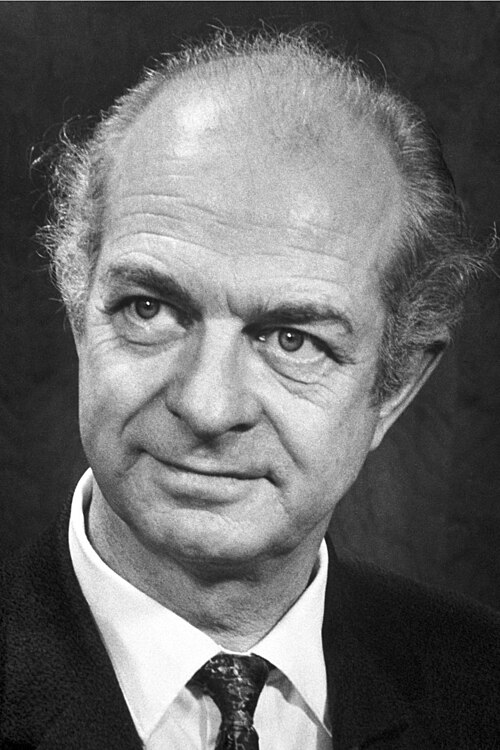
\includegraphics[width=0.24\linewidth]{images/book2/pauling.jpg}

{\small लाइनस पॉलिंग (1901--1994)।}
\end{omfigure}

\section{रासायनिक लक्षण की प्रवृत्तियाँ}

\begin{proposition}[अपचायक और ऑक्सीकारक लक्षण]\label{prop:b1:periodicity:redox-trend}
कम आयनन ऊर्जा और कम \omterm{def:b1:periodicity:electronegativity}{विद्युत-ऋणात्मकता} वाले तत्व, जो सारणी के बाईं ओर
और अपने समूहों के निचले भाग में हैं, आसानी से इलेक्ट्रॉन खोते हैं:
वे अपचायक धातुएँ हैं (सबसे अधिक क्षार धातुएँ)। उच्च
\omterm{def:b1:periodicity:electronegativity}{विद्युत-ऋणात्मकता} और \omterm{def:b1:periodicity:electron-affinity}{इलेक्ट्रॉन बंधुता} वाले तत्व, जो ऊपर दाईं ओर हैं, आसानी से
इलेक्ट्रॉन ग्रहण करते हैं: वे ऑक्सीकारक अधातुएँ हैं (सबसे अधिक फ़्लुओरीन, ऑक्सीजन
और क्लोरीन)। उत्कृष्ट गैसें, उच्च आयनन ऊर्जा और अतिरिक्त
इलेक्ट्रॉन के प्रति किसी बंधुता के बिना, दोनों में से कुछ नहीं करतीं।
\end{proposition}

\begin{method}[स्थिति से प्रवृत्ति का अनुमान]\label{met:b1:periodicity:predict}
दो तत्वों की तुलना ऐसे गुण के लिए करने हेतु जो \omterm{def:b1:quantum-numbers:configuration}{संयोजकता इलेक्ट्रॉनों} पर
नाभिक की पकड़ से जुड़ा है (त्रिज्या, $E_i$, $E_{ea}$, $\chi$):
\begin{enumerate}
  \item यदि वे एक ही समूह में हैं, तो नीचे वाले का
        $n$ बड़ा है: बड़ी त्रिज्या, कम $E_i$ और $\chi$;
  \item यदि वे एक ही \omterm{def:b1:periodicity:table}{आवर्त} में हैं, तो अधिक दाईं ओर वाले का
        $Z^{*}$ बड़ा है: छोटी त्रिज्या, अधिक $E_i$ और $\chi$;
  \item अन्यथा हर एक की तुलना उस तत्व से कीजिए जो उसकी पंक्ति और दूसरे के
        स्तंभ के मिलन-बिंदु पर है;
  \item आयनन ऊर्जाओं पर निष्कर्ष निकालने से पहले \omterm{def:b1:quantum-numbers:orbital}{उपकोश} प्रभावों (p \omterm{def:b1:quantum-numbers:orbital}{उपकोश} का
        आरंभ, पहला युग्मित p इलेक्ट्रॉन) की जाँच कीजिए।
\end{enumerate}
\end{method}

\begin{example}[बैटरी में लीथियम]\label{ex:b1:periodicity:lithium}
\omterm{def:b1:periodicity:table}{आवर्त} 2 में लीथियम की \omterm{def:b1:periodicity:electronegativity}{विद्युत-ऋणात्मकता} सबसे कम है और वह अपना 2s
इलेक्ट्रॉन आसानी से खो देता है, जबकि वह सबसे हल्की धातु है: किसी भी तत्व की तुलना में
प्रति ग्राम सबसे अधिक स्थानांतरणीय आवेश वही ढोता है, और इसी कारण वह
पुनः आवेशनीय बैटरियों को ऊर्जा देता है। उसकी \omterm{def:b1:periodicity:ionisation-energy}{प्रथम आयनन ऊर्जा}, \qty{5.39}{eV},
सोडियम (5.14) या पोटैशियम (4.34) से अधिक है, फिर भी पानी में वह
सबसे प्रबल अपचायक क्षार धातु है; यह विरोधाभास छोटे \ce{Li+} आयन के प्रबल
जलयोजन से सुलझता है (\cref{ch:b1:nernst})।
% ledger: ie:Li, ie:Na, ie:K
\end{example}

\section{अभ्यास}

\begin{exercise}[$\star$]\label{exo:b1:periodicity:1}
कैल्सियम, आयरन, सेलेनियम और आयोडीन ($Z = 20, 26, 34, 53$) के विन्यासों से
उनका \omterm{def:b1:periodicity:table}{आवर्त}, समूह और \omterm{def:b1:periodicity:table}{ब्लॉक} बताइए।
\end{exercise}

\begin{exercise}[$\star$]\label{exo:b1:periodicity:2}
हर जोड़े में कौन-सी स्पीशीज़ बड़ी है, और क्यों? \ce{Na} या \ce{Cl};
\ce{Na} या \ce{Na+}; \ce{F-} या \ce{Cl-}; \ce{Na+} या \ce{Mg^{2+}}।
\end{exercise}

\begin{exercise}[$\star$]\label{exo:b1:periodicity:3}
\ce{Na}, \ce{Mg}, \ce{Al}, \ce{P},
\ce{S} और \ce{Ar} की \omterm{def:b1:periodicity:ionisation-energy}{प्रथम आयनन ऊर्जाएँ} 5.14, 7.65, 5.99, 10.49, 10.36 और
\qty{15.76}{eV} हैं। इन्हें क्रम में रखिए और सामान्य प्रवृत्ति से दो विचलन
बताइए।
\end{exercise}

\begin{exercise}[$\star$]\label{exo:b1:periodicity:4}
किसी स्पीशीज़ की \omterm{def:b1:periodicity:polarisability}{ध्रुवणीयता} की परिभाषा दीजिए। कौन अधिक ध्रुवणीय है, \ce{F-}
या \ce{I-}? \ce{Na+} या \ce{Cl-}? कारण बताइए।
\end{exercise}

\begin{exercise}[$\star\star$]\label{exo:b1:periodicity:5}
\omterm{def:b1:periodicity:table}{आवर्त} 3 के किसी तत्व की पहली चार आयनन ऊर्जाएँ 5.99,
18.83, 28.45 और \qty{119.99}{eV} हैं। क्रमिक अनुपात परिकलित कीजिए, और
तत्व तथा उसके द्वारा बनाए जाने वाले आयन को पहचानिए।
\end{exercise}

\begin{exercise}[$\star\star$]\label{exo:b1:periodicity:6}
समझाइए कि क्लोरीन की \omterm{def:b1:periodicity:electron-affinity}{इलेक्ट्रॉन बंधुता} फ़्लुओरीन से अधिक क्यों है, और
नाइट्रोजन तथा मैग्नीशियम कोई स्थायी गैसीय ऋणायन क्यों नहीं बनाते।
\end{exercise}

\begin{exercise}[$\star\star$]\label{exo:b1:periodicity:7}
सोडियम ($E_{i1} =
\qty{5.14}{eV}$, $E_{ea} = \qty{0.55}{eV}$) और क्लोरीन ($E_{i1} =
\qty{12.97}{eV}$, $E_{ea} = \qty{3.61}{eV}$) की मुलिकेन \omterm{def:b1:periodicity:electronegativity}{विद्युत-ऋणात्मकताएँ} परिकलित
कीजिए। ये \ce{NaCl} के आबंध के बारे में क्या बताती हैं?
\end{exercise}

\begin{exercise}[$\star\star$]\label{exo:b1:periodicity:8}
\cref{ex:b1:periodicity:bonds} के पॉलिंग मानों और $\chi(\ce{F})
= 3.98$ की सहायता से आबंधों \ce{H-F}, \ce{C-H}, \ce{Na-Cl}, \ce{C-Cl}
($\chi(\ce{Cl}) = 3.16$) और \ce{O-H} का वर्गीकरण कीजिए, और हर परमाणु पर
आंशिक आवेश का चिह्न बताइए।
\end{exercise}

\begin{exercise}[$\star\star$]\label{exo:b1:periodicity:9}
\ce{Li}, \ce{Na} और \ce{K} की \omterm{def:b1:periodicity:ionisation-energy}{प्रथम आयनन ऊर्जाएँ} 5.39,
5.14 और \qty{4.34}{eV} हैं। प्रवृत्ति समझाइए और अनुमान लगाइए कि
रुबिडियम की ऊर्जा \qty{4.34}{eV} से ऊपर है या नीचे।
\end{exercise}

\begin{exercise}[$\star\star\star$]\label{exo:b1:periodicity:10}
ज़िंक ($Z = 30$) की \omterm{def:b1:periodicity:ionisation-energy}{प्रथम आयनन ऊर्जा} \qty{9.39}{eV} है और
गैलियम ($Z = 31$) की \qty{6.00}{eV}; आर्सेनिक ($Z = 33$) की \qty{9.79}{eV}
और सेलेनियम ($Z = 34$) की \qty{9.75}{eV}। विन्यासों की सहायता से दोनों गिरावटें
समझाइए।
\end{exercise}

\begin{exercise}[$\star\star\star$]\label{exo:b1:periodicity:11}
$D(\ce{H-H}) = \qty{436}{kJ/mol}$, $D(\ce{F-F}) =
\qty{158}{kJ/mol}$, $\chi(\ce{H}) = 2.20$ और $\chi(\ce{F}) = 3.98$ लीजिए, साथ में
$\qty{1}{eV} = \qty{96.5}{kJ/mol}$। पॉलिंग की परिभाषा से
आबंध ऊर्जा $D(\ce{H-F})$ का अनुमान लगाइए। यह दोनों सममित आबंधों के माध्य से
इतनी अधिक क्यों है?
\end{exercise}

\begin{exercise}[$\star\star\star$]\label{exo:b1:periodicity:12}
क्रिप्टॉन (3.00) और ज़ेनॉन (2.60) की पॉलिंग \omterm{def:b1:periodicity:electronegativity}{विद्युत-ऋणात्मकताएँ} सारणीबद्ध हैं,
पर हीलियम, नियॉन या आर्गन की नहीं। पैमाने की परिभाषा
से समझाइए कि मान केवल ऐसे तत्व के लिए क्यों दिया जा सकता है जो आबंध
बनाता है, और भारी उत्कृष्ट गैसें ही आबंध क्यों बनाती हैं।
% ledger: en:Kr, en:Xe
\end{exercise}

\section{समस्या: पॉलिंग का अंकगणित}

\begin{problem}[{सप्ताहांत समस्या --- आयनन ऊर्जाओं से एक अज्ञात तत्व,
समान आकार के मेघ वाले आयनों की एक श्रेणी, विद्युत-ऋणात्मकता के दो पैमाने,
और H--Cl आबंध के लिए पॉलिंग की संख्या}]
\label{pb:b1:periodicity:1}
आँकड़े: प्रति कण $\qty{1}{eV}$, \qty{96.485}{kJ/mol} के संगत है।

\medskip
\noindent\textbf{भाग I --- एक अज्ञात तत्व।}
\omterm{def:b1:periodicity:table}{आवर्त} 3 के एक तत्व X की पहली चार आयनन ऊर्जाएँ 7.65,
15.04, 80.14 और \qty{109.27}{eV} हैं।
\begin{enumerate}
  \item हर आयनन ऊर्जा पिछली से बड़ी क्यों है?
  \item अनुपात $E_{i2}/E_{i1}$, $E_{i3}/E_{i2}$ और
        $E_{i4}/E_{i3}$ परिकलित कीजिए।
  \item X का समूह निकालिए, फिर उसे पहचानिए।
  \item X अपने यौगिकों में कौन-सा आयन बनाता है? उसका विन्यास बताइए।
  \item X धातु है या अधातु? उसकी स्थिति से कारण बताइए।
  \item तीसरा इलेक्ट्रॉन दूसरे से इतना अधिक महँगा क्यों है?
\end{enumerate}

\medskip
\noindent\textbf{भाग II --- दस इलेक्ट्रॉन।}
\ce{O^{2-}}, \ce{F-}, \ce{Na+},
\ce{Mg^{2+}} और \ce{Al^{3+}} की \omterm{def:b1:periodicity:radius}{आयनिक त्रिज्याएँ} (छह पड़ोसी) 140, 133, 102, 72 और \qty{54}{pm} हैं।
\begin{enumerate}[resume]
  \item दिखाइए कि इन आयनों का विन्यास एक ही है।
  \item त्रिज्याओं का क्रम समझाइए।
  \item पाँचों आयनों में कौन सबसे अधिक ध्रुवणीय है, और क्यों?
  \item सबसे बड़ी और सबसे छोटी त्रिज्या का अनुपात परिकलित कीजिए।
  \item \ce{Cl2} की आबंध लंबाई \qty{198.8}{pm} है और
        \ce{Cl-} की त्रिज्या \qty{181}{pm}। क्लोरीन की \omterm{def:b1:periodicity:radius}{सहसंयोजी त्रिज्या} परिकलित कीजिए
        और तुलना कीजिए।
  \item बिना और आँकड़ों के, \ce{Cl-}, \ce{Na+} और \ce{Mg^{2+}} को
        आकार के क्रम में रखिए।
\end{enumerate}

\medskip
\noindent\textbf{भाग III --- मुलिकेन का पैमाना।}
\begin{center}
\small
\begin{tabular}{lccccc}
\hline
तत्व & \ce{F} & \ce{Cl} & \ce{Br} & \ce{O} & \ce{C} \\
\hline
$E_{i1}$ (eV) & 17.42 & 12.97 & 11.81 & 13.62 & 11.26 \\
$E_{ea}$ (eV) & 3.40 & 3.61 & 3.36 & 1.44 & 1.26 \\
पॉलिंग $\chi$ & 3.98 & 3.16 & 2.96 & 3.44 & 2.55 \\
\hline
\end{tabular}
\end{center}
% ledger: ie:F, ie:Cl, ie:Br, ie:O, ie:C, ea:F, ea:Cl, ea:Br, ea:O, ea:C,
% en:F, en:Cl, en:Br, en:O, en:C
\begin{enumerate}[resume]
  \item पाँचों तत्वों की मुलिकेन \omterm{def:b1:periodicity:electronegativity}{विद्युत-ऋणात्मकताएँ} परिकलित कीजिए।
  \item दोनों पैमानों पर इन्हें क्रम में रखिए। कौन-सा तत्व भिन्न स्थान पाता है?
  \item तीनों हैलोजनों के लिए अनुपात $\chi_{\text{पॉलिंग}}/\chi_M$ परिकलित
        कीजिए। आप क्या देखते हैं?
  \item सुझाइए कि ऑक्सीजन हैलोजनों के नियम से क्यों हटता है (उसकी
        \omterm{def:b1:periodicity:electron-affinity}{इलेक्ट्रॉन बंधुता} देखिए)।
  \item \ce{HCl} में आंशिक ऋणात्मक आवेश किस परमाणु पर है? और
        \ce{ClF} में?
  \item सारणीबद्ध मानों ($\chi(\ce{H}) = 2.20$) के साथ, क्या \ce{H-Cl}
        आबंध अध्रुवीय है, ध्रुवीय सहसंयोजी है या आयनिक?
\end{enumerate}

\medskip
\noindent\textbf{भाग IV --- H--Cl के लिए पॉलिंग की संख्या।}
\qty{298}{K} पर \ce{H(g)}, \ce{Cl(g)} और
\ce{HCl(g)} की मानक विरचन एन्थैल्पियाँ 218.0, 121.3 और \qty{-92.3}{kJ/mol} हैं;
\ce{H2(g)} और \ce{Cl2(g)} की शून्य हैं। किसी
अणु की आबंध ऊर्जा को उसके परमाणुओं में वियोजन की एन्थैल्पी माना जाता है।
% ledger: janaf:H, janaf:Cl, janaf:HCl
\begin{enumerate}[resume]
  \item $D(\ce{H-H})$ को \ce{H2(g) -> 2H(g)} से परिकलित कीजिए।
  \item $D(\ce{Cl-Cl})$ परिकलित कीजिए।
  \item $D(\ce{H-Cl})$ को \ce{HCl(g) -> H(g) + Cl(g)} से परिकलित कीजिए।
  \item पॉलिंग की अतिरिक्त ऊर्जा $\Delta E$ kJ/mol में परिकलित कीजिए, और दिखाइए
        कि यह $-\Delta_f H(\ce{HCl})$ के बराबर है।
  \item $\Delta E$ को इलेक्ट्रॉनवोल्ट में बदलिए।
  \item $|\chi(\ce{Cl}) - \chi(\ce{H})|$ परिकलित कीजिए और उसकी तुलना
        सारणीबद्ध मानों के अंतर, $3.16 - 2.20$, से कीजिए।
\end{enumerate}
\end{problem}
